Adaptivity is supported through usage of the Percept module. However, this code base has not yet
been deployed to the open sector. As such, ifdef gaurds are placed within the code base. A variety of 
choices exist for the manner by which hanging nodes are removed in a vertex-centered code base.

A typical h-adapted patch of elements
is shown in Figure~\ref{hadapt-convol}.  The ``hanging nodes"
do not have control volumes associated with them.  Rather,
they are constrained to be a linear combination of the
two parent edge nodes.  There is no element assembly procedure 
to compute fluxes for the ``hanging sub-faces" associated with the hanging 
nodes that occur along the parent-child element boundary.

\begin{figure}[h]
  \centerline{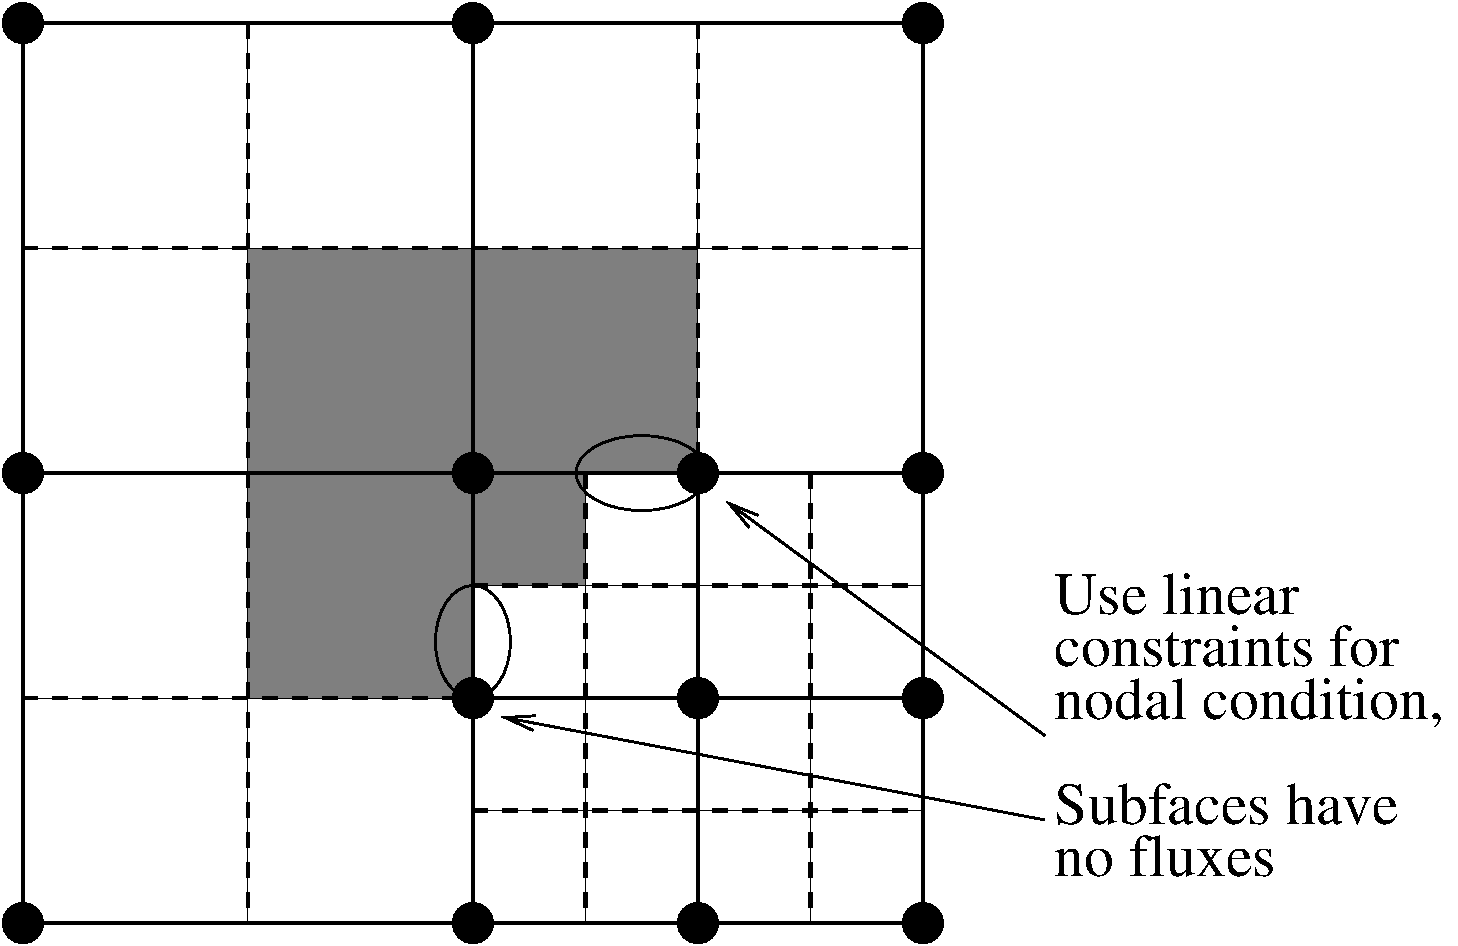
\includegraphics[width=5.5in]{images/hadapt.pdf}}
  \vspace{0.25in}
  \caption{Control volume definition on an h-adapted mesh
           with hanging nodes. (Four-patch of parent elements 
           with refinement in bottom-right element.) }
  \label{hadapt-convol}
\end{figure}

\noindent
In general, for a vertex-centered scheme, the h-adaptive scheme is driven at the element level.
Refinement occurs within the element and the topology of refined elements is the same as the parent element. 

Aftosmis~\cite{Aftosmis:94} describes a vertex-centered
finite-volume scheme on unstructured Cartesian meshes.
A transitional set of control volumes are formed about
the hanging nodes, shown in Figure~\ref{aftosmis-convol}.  
on unstructured meshes. This approach would require a
series of specialized master elements to deal with the
different transition possibilities.

\begin{figure}[h]
  \centerline{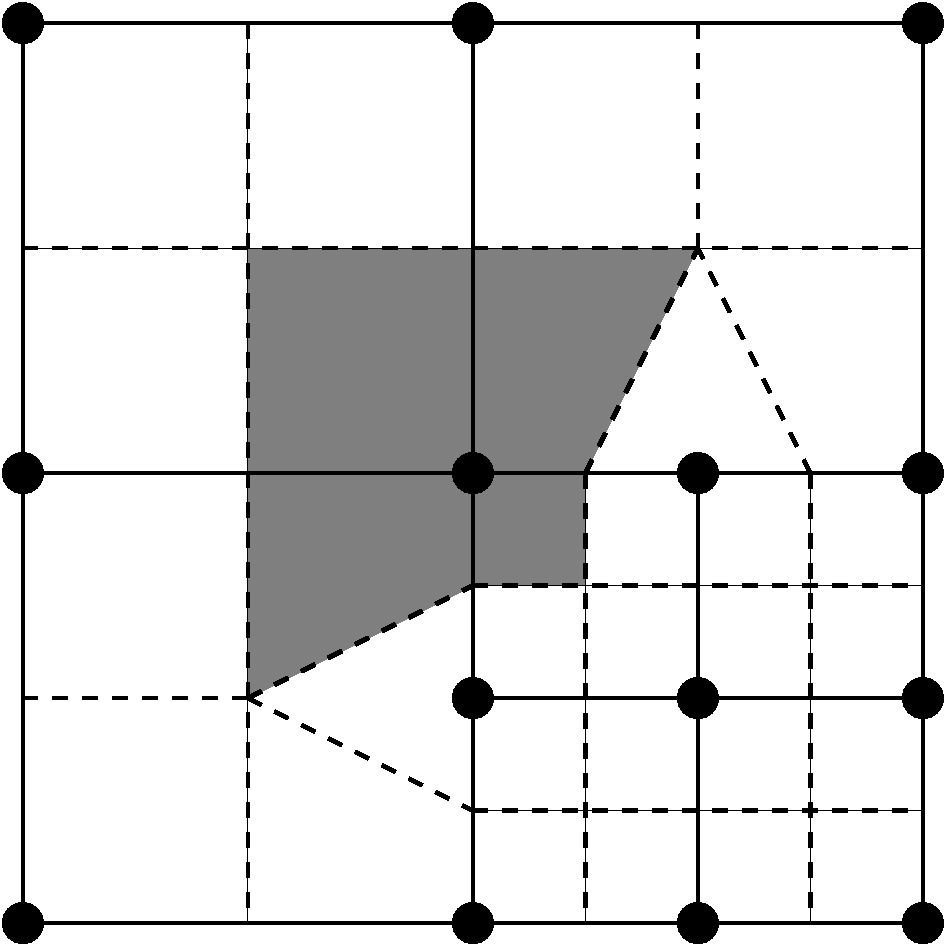
\includegraphics[width=3.5in]{images/hadapt2.pdf}}
  \vspace{0.25in}
  \caption{Control volume definition on an h-adapted mesh
           with transition control volumes about the
           hanging nodes. (Four-patch of parent elements 
           with refinement in bottom-right element.) }
  \label{aftosmis-convol}
\end{figure}

Kallinderis~\cite{Kallinderis:89} describes a vertex-centered
finite-volume scheme on unstructured quad meshes.  Hanging
nodes are treated with a constraint condition.  The flux
construction for a node on a refinement boundary is based
on the unrefined parent elements, leading to a 
non-conservative scheme.

Kallinderis~\cite{kallinderis:93} also describes a vertex-centered
finite-volume scheme on unstructured tetrahedral meshes.  Hanging
nodes are removed by splitting the elements on the ``unrefined"
side of the refinement boundary. Mavriplis~\cite{Mavriplis:00} uses a similar 
technique, however, extends it to a general set of heterogeneous elements,
shown in Figure~\ref{kallin-convol}.

\begin{figure}[h]
  \centerline{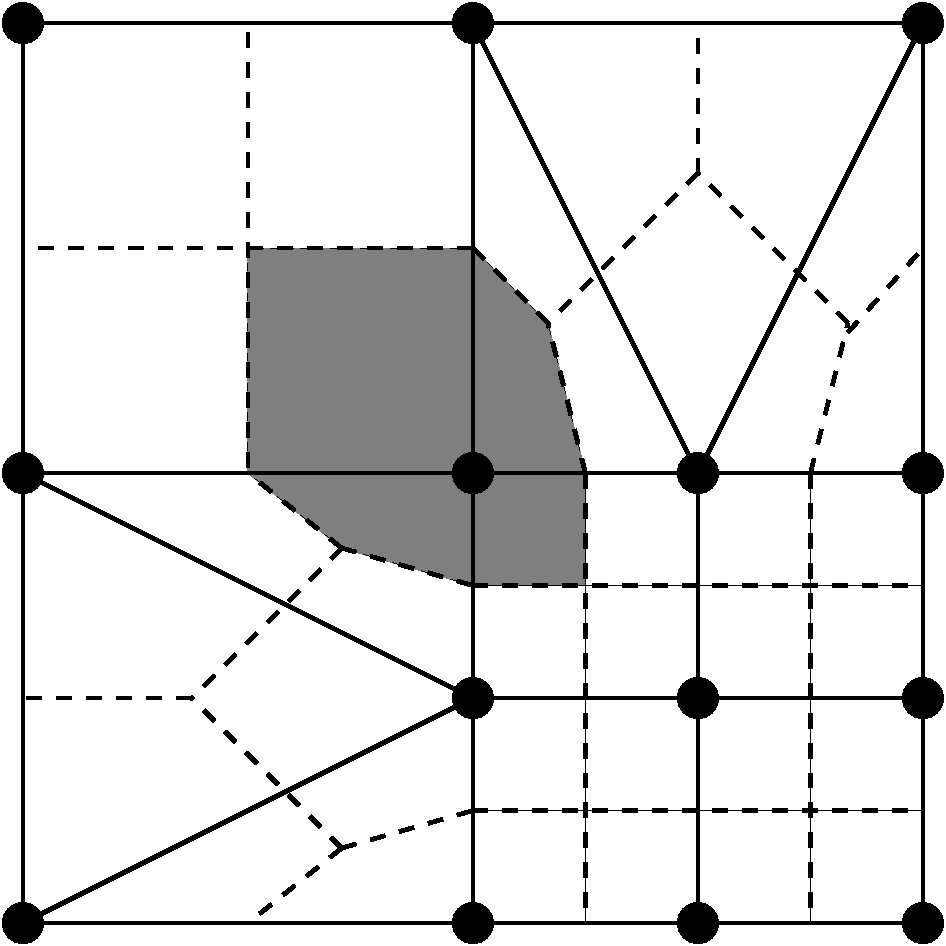
\includegraphics[width=3.5in]{images/hadapt3.pdf}}
  \vspace{0.25in}
  \caption{Control volume definition on a heterogeneous
           h-adapted mesh with no hanging nodes.
           (Four-patch of parent elements 
           with refinement in bottom-right element
           and splitting in adjacent parent elements.) }
  \label{kallin-convol}
\end{figure}

The future deployment of Percept will use the procedure of Mavriplis whereby hanging 
nodes are removed by neighbor topological changes. A variety of error indicators exists 
and a prototyped error transport equation appraoch for the one-equation $k^{sgs}$ model 
has been tested for classic jet-in-crossflow configurations.

\subsection{Prolongation and Restriction}

Nodal variables are interpolated between levels of the
h-adapted mesh hierarchy using the traditional prolongation
and restriction operators defined over an element.  The
prolongation operation is used to compute values for new
nodes that arise from element sub-division.  The parent element
shape functions are used to interpolate values from the parent
nodes to the sub-divided nodes.

Prolongation and restriction operators for element variables and 
face variables are required to maintain mass flow rates that
satisfy continuity. When adaptivity takes place, a code option
to reconstruct the mass flow rates must be used. Whether or not
a Poisson system must be created has been explored. More work is 
required to understand the nuances associated with prolongation, 
specifically with respect to possible dispersion errors.
